\chapter{Enlace cristalino}

En este capítulo se estudian los distintos mecanismos de \textit{cohesión} de los cristales. La \textit{distribución electrónica} alrededor de los núcleos caracteriza, a nivel microscópico, el tipo de enlace cristalino: \textit{covalente, metálico, molecular, iónico} y \textit{de hidrógeno}. La \textit{energía de cohesión} (aquella que se debe suministrar al cristal para separarlo en sus constituyentes) varía para los elementos cristalinos desde 0.02 eV/átomo en el Ne hasta 8.9 en el W.

\section{Clasificación de los sólidos}

El cálculo de la energía de cohesión requiere el conocimiento de los estados electrónicos en el cristal. Las funciones de onda electrónicas de los electrones de valencia de los átomos libres cambian (y en consecuencia la distribución de carga) cuando los átomos se unen formando el cristal. En función de cuánto cambian estos estados electrónicos, los sólidos suelen clasificarse en cuatro tipos fundamentales, con distribuciones electrónicas según muestra la figura :

\begin{itemize}
    \item \textbf{Moleculares}: con cambio mínimo.
    \item \textbf{Iónicos} en los que hay trasferencia de carga.
    \item \textbf{Covalentes} en los que la distribución de carga es direccional y localizada.
    \item \textbf{Metálicos} con carga electrónica extendida a todo el cristal.
\end{itemize}

\section{Cristales moleculares}

Son aquellos en que los nudos están ocupados por moléculas en las que los \textit{enlaces intermoleculares son débiles} (al menos respecto los intramoleculares). Ejemplo de estos son los gases inertes y gases orgánicos (metano...). Los átomos de gases inertes tienen las capas electrónicas cerradas con simetría esférica. La baja energía de ionización ($\sim 1 \%$) sugiere que la distribución de carga no se distorsiona apreciablemente. 


\subsection{Interacción de \textit{van der Waals-London}}

La deformación atómica más sencilla que conduce a una interacción no nula entre átomos es el desplazamiento de la nube electrónica (\textit{rígida}) de manera que aparezca un momento dipolar. El modelo simple que muestra en la figura en el que se supone $x_1,x_2\ll R$, permite dar cuenta de la existencia de una interacción atractiva entre átomos o moléculas neutros. 

La energía de los dos osciladores sin interacción ($R\rightarrow \infty$) esférica

\begin{equation}
    H_0 = \frac{p_1^2}{2M} + \frac{1}{2} Cx_1^2 + \frac{p_2^2}{2M} + \frac{1}{2} Cx_2^2
\end{equation}
donde $C=M\omega_0^2$ siendo $\omega_0$ la frecuencia propia de vibracción de la carga (rígida) negativa de los átomos y $M$ su masa. Por su parte, la energía de interacción de Coulomb se expresa por 

\begin{equation}
    H_i = \frac{q^2}{R} + \frac{q^2}{R+x_1-x_2} - + \frac{q^2}{R+x_1} - + \frac{q^2}{R-x_2} \approx - \frac{2q^2x_1x_2}{R^3}
\end{equation}
donde $q^2=e^2$ en unidades cgs o $q^2 = e^2 / 4\pi \epsilon_0$ en mks. El hamiltoniano total $H=H_0+H_i$ se puede diagonalizar para obtener sus valores propios, introduciendo las llamadas {\it variables normales}

\begin{align}
    x_s \equiv \frac{1}{\sqrt{2}} (x_1 + x_2)  \tquad  & x_a \equiv \frac{1}{\sqrt{2}} (x_1-x_2) \\
    p_s \equiv \frac{1}{\sqrt{2}} (p_1 + p_2) \tquad & p_a \equiv \frac{1}{\sqrt{2}} (p_1-p_2) 
\end{align}
de modo que 

\begin{equation}
    H = \ccorchetes{\frac{p_s^2}{2M}+ \frac{1}{2} \parentesis{C- \frac{2q^2}{R^3}}x_s^2} + \ccorchetes{\frac{p_a^2}{2M}+ \frac{1}{2} \parentesis{C+ \frac{2q^2}{R^3}}x_a^2} 
\end{equation}
Formalmente el problema se reduce al de dos \textit{osciladores} independientes, de frecuencias propias:

\begin{equation}
\omega_s^2 = \omega_0^2 - \frac{2q^2}{MR^3} \quad \omega_a^2 = \omega_0^2 + \frac{2q^2}{MR^3}
\end{equation}
El cambio en la energía (por oscilador) debido al acoplamiento será $\Delta E = \frac{1}{2} (\hbar \omega_s + \hbar \omega_a - 2 \hbar \omega_0$), qe en la aproximación  $ \frac{2q^2}{MR^3} \ll \omega_0^2$ es

\begin{equation}
\Delta E \approx - \frac{1}{2} \hbar \omega_0 \parentesis{\frac{q^2}{CR^3}}^2 \propto -C^{-3/2}  R^{-6} \label{Ec:03-02-07}
\end{equation}
La dependencia (\ref{Ec:03-02-07}) coincide con la clásica \textit{dipolo-dipolo inducido}. Observar sin embargo que la interacción es un efecto cuántico en cuanto que $\Delta E \rightarrow 0$ si $\hbar \rightarrow 0$. 

\textbf{Interacción repulsiva}. Además de la \textit{repulsión electroestática} entre las nubes electrónicas, el \textit{Principio de Pauli} impide que átomos con capas llenas puedan solaparse a menos que haya promoción parcial de los electrones a estados energéticos más altos desocupados (lo cual implicaría un costo de energía). Es de esperar entonces que la interacción repulsiva sea de corto alcance y, en efecto, los datos experimentales de los gases inertes pueden ajustarse bien por un potencial \textit{semiempírico} con dependencia de la separación entre átomos según $R^{-12}$.

\subsection{Interacción de Lennard-Jones}


El potencial de interacción por par de átomos $i$ y $j$ (a distancia $r_{ij}$) resultante (contribución atractiva más repulsiva) puede escribirse Coulomb

\begin{equation}
    U (r_{ij}) = 4 \epsilon \ccorchetes{\parentesis{\frac{\sigma}{r_{ij}}}^{12}-\parentesis{\frac{\sigma}{r_{ij}}}^6}
\end{equation}
Esta ecuación describe la llamada \textbf{intearcción de Lennard-Jones} o  \textbf{interacción 6-12}. Es una función experimental que describe muy bien cierto tipo de sólidos. Los parámetros $\epsilon$ y $\sigma$ pueden determinarse a partir de medidas de viscosidad y coeficientes de virial en la fase gaseosa. El potencial total sobre un átomo $i$ cualquiera esférica

\begin{equation}
    U_i = \sum_{j\neq i}^N U(r_{ij}) = 4 \epsilon \ccorchetes{B \parentesis{\frac{\sigma}{R}}^{12}-A\parentesis{\frac{\sigma}{R}}^6} \quad \text{con} \ B = \sum_{i\neq j}^N p_{ij}^{-12} \quad A = \sum_{i\neq j}^N p_{ij}^{-6} 
\end{equation}
siendo $R$ la distancia entre vecinos más proximos y $p_{ij}=r_{ij}/R$. Las sumas $A$ y $B$ dependen de la estructura cristalina. En el cuadro \ref{Tab:03-01} (izquierda) se dan sus valores para algunas de las más comunes.

\begin{figure}[h!] \centering
    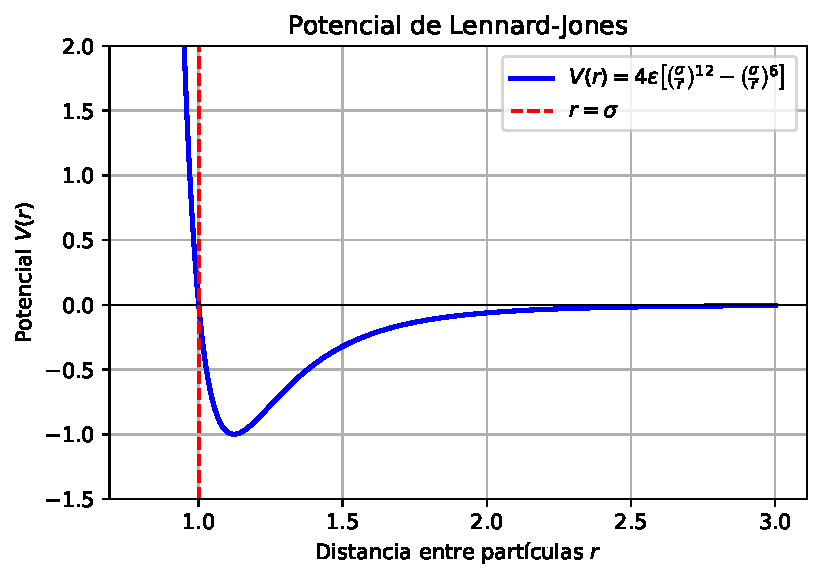
\includegraphics[scale=1.05]{Cuerpo/Ch_03/Lennard-jones.pdf}
    \caption{Potencial de Lennard-jones para variables reducidas ($\epsilon,\sigma = 1$)}
    \label{Fig:03-03}
\end{figure}    

El potencial total del cristal resulta

\begin{equation}
    U = \frac{1}{2} \sum_i^N U_i = 2 \epsilon N \ccorchetes{B\parentesis{\frac{\sigma}{R}}^{12}-A\parentesis{\frac{\sigma}{R}}^6} \label{Ec:03-02-10}
\end{equation}
A partir de la ecuación \ref{Ec:03-02-10} se puede calcular la distancia de equilibrio $R_0$ por la condición $(\D U / \D R)_{R_0} =0$ obteniéndose $R_0 / \sigma = (2B/A)^{1/6}$ (1.09 para una estructura \textit{fcc}). Los valores experimentales para algunos gases nobles (\textit{fcc}) son los mostrados en el cuadro  \ref{Tab:03-01} (derecha). La pequeña desviación de los átomos más ligeros se debe a \textit{efectos cuánticos del punto cero}. Esto se entiende por el espacio de confinamiento del átomo en el cristal, la energía cinética será $p^2/2m= (h/\lambda)^2/2m$: inversamente proporcional a la masa. 

En cuanto a la energía de cohesión (en equilibrio) a temperatura cero se puede obtener sin más que sustituir en \ref{Ec:03-02-10} $R=R_0$ resultando

\begin{equation}
U_0 \equiv (R_0) = - N\epsilon (A^2/2B)
\end{equation}
La estructura con menor $U_0$ es la \textit{fcc} ($-8.6 N\epsilon$), que es la que tienen todos los cristales de gases nobles. Las correciones mecanocuánticas a $U_0$ alcanzan casi un 30\% en el Ne y hasta un  4\% en el Xe.

\begin{table}[h!] \centering
\begin{tabular}{ccccccccc}
Estructura & B & A & & Elemento & Ne & Ar & Kr & Xe \\ \cline{1-3} \cline{5-9} 
\fcc & 12.122 & 14.454 & \quad & $R_0/\sigma$ & 1.14 & 1.11 &1.10 & 1.09 \\
\hcp & 12.132 & 14.455 & & $-U/N\epsilon$ & 5.59 & 8.24 & 8.61 & 8.62 \\
\bcc & 9.114 & 12.253 & & $-U_0 (\unit{\eV}/\text{at.})$ & 0.02 & 0.08 & 0.12 & 0.17\end{tabular}
\caption{A la izquierda los parámetros A y B para las estrucutras indicadas. A la derecha valores experimentales para los cristales de gases nobles con estrucutra \fcc.}
\label{Tab:03-01}
\end{table}

\section{Cristales iónicos}
Son los formados por iones positivos y negativos. El enlace iónico es fuerte (6-12 eV/ion) y es el resultado de la interacción electroestática \textit{directa} de iones con \textit{capas electrónicas completas}, como por ejemplo el $\Namas$ ($1s^22s^2 2p^6)$ y $\Clmenos$ ($1s^22s^2 2p^6 3s^2 3p^6$).

\textbf{Constante de Madelung.} Aparece al calcular la energía (potencial) de cohesión de un cristal iónico admitiendo una energía potencial por pares de forma 

\begin{equation}
    U_{ij} = \frac{\pm q^2}{r_{ij}} + \frac{B}{r_{ij}^n} \label{Ec:03-03-01}
\end{equation} 
donde $B$ y $n$ ($n\gg 1$) son desconocidos ($q^2 = e^2$ en unidades cgs o $q^2=e^2 / 4 \pi \epsilon_0$ en mks). Otra aproximación válida sería utilizar una intersección repulsiva de la forma $\lambda e^{-r_{ij}/\rho}$. Análogamente a las sumas en \ref{Ec:03-02-10}, al sumar \ref{Ec:03-03-01} para todos los pares (N átomos) se tiene 

\begin{equation}
    U = \frac{N}{2} \parentesis{\frac{BA_n}{R^n}-\frac{\alpha q^2}{R}}
\end{equation}
con 

\begin{equation}
    A_n = \sum_{i\neq j} p_{ij}^{-n} \tquad \alpha = \sum_{j \neq i} \pm p_{ij}^{-1} \quad p_{ij} = \frac{r_{ij}}{R}
\end{equation}
tal que a $\alpha$ se conoce como \textbf{constante de Madelung} y su valor depende de la estructura (cuadro \ref{Tab:03-02}).

\begin{table}[h!] \centering
    \begin{tabular}{c|ccc}
        Estrucura & ClNa & ClCs & ZnS cúbica \\ \hline
        $\alpha$ & 1.748 & 1.763 & 1.638 
    \end{tabular}
    \caption{Constante de Madelung para algunas estructuras muy comunes.}
    \label{Tab:03-02}
\end{table}

La separación de equilibrio $R_0$ se calcula a partir  de la condición $(\partial U / \partial R)_{R_0} = 0 \Rightarrow R_0 = (nBA_n/\alpha q^2)^{1//(n-1)}$, a la cual

\begin{equation}
U(R_0) = - \frac{N}{2} \frac{\alpha q^2}{R_0} \parentesis{1-\frac{1}{n}} \label{Ec:03-03-04}
\end{equation}
El exponente $n$ puede relacionarse con el coeficiente de compresibilidad $K\equiv - V^{-1}(\partial V / \partial P)_{R_0}$ (donde $P$ es la presión y $V$ el volumen) según $n=1+18R_0^4 / Kq^2 \alpha$. Como ejemplo para el NaCl (\fcc), a partir del valor experimental $K=3.3\times 10^{-12} \unit{\cm}^2 / \text{dyna}$ hy $\alpha = 1.75$ se obtiene $n=9.4$. También para el NaCl se obtiene que $\rho=0.3 \ \unit{\angstrom}$ admitiendo una forma exponencial para la interacción repulsiva, de modo que resulta ser ésta de muy corto alcance.

Las energías de cohesión de cristales iónicos típicos como los haluros alcalinos se predicen según ecuación \ref{Ec:03-03-04}, con una precisión mejor que el 10\%. El término $-N\alpha q^2 / 2 R_0$ representa prácticamente el 90\% de $U(R_0)$ . En el cuadro se dan estos valores para  algunos \textit{haluros alcalinos}.

\begin{table}[h!] \centering
    \begin{tabular}{c|ccccc}
        & Li & Na & K & Rb & Cs \\ \hline
        F & 10.5 & 9.31 & 8.25 & 7.86 & 7.50 \\
          & \textbf{12.6} & \textbf{10.9} & \textbf{9.44} & \textbf{8.94} & \textbf{8.38} \\ \hline
        Cl & 8.63  & 7.94 & 7.19 & 6.94 & \\
           & \textbf{9.82} & \textbf{8.94} & \textbf{8.00} & \textbf{7.69} & \\ \hline  
        Br & 8.25 & 7.56 & 6.86 & 6.63 & \\
           & \textbf{9.19} & \textbf{8.44} & \textbf{7.63} & \textbf{7.38} & \\ \hline
        I & 7.69 & 7.06 & 6.50 & 6.31 & \\
        & \textbf{8.38} & \textbf{7.75} & \textbf{7.13} & \textbf{6.88} &  
    \end{tabular}
    \caption{Energía de cohesión experimental (eV/par-de-iones). En negrita la energía de cohesión teórica considerando sólo el término $N\alpha q^2 / 2 R_0$.}
\end{table}

\section{Cristales covalentes}

El enlace covalente entre dos átomos, muy común en los compuestos orgánicos, involucra a sendos a electrones de valencia  que son compartidos. Este \textit{solapamiento} asociado de carga electrónica en la dirección de la unión de los átomos genera un enlace fuerte (7.3 eV/átomo en el diamante). Los cristales covalentes suelen ser duros y quebradizos.

\subsection{La molécula ion de hidrógeno $H_2^+$}

Esta molécula ilustra lo esencial del enlace covalente y admite solución exacta minimizando $\langle E \rangle = \langle \Psi | H | \Psi \rangle$ donde 

\begin{equation*}
    H = - \frac{\hbar^2}{2m} \Delta - \frac{q^2}{r_a} - \frac{q^2}{r_b} + \frac{q^2}{R}
\end{equation*}
es el Hamiltoniano del electrón y los dos núcleos, supuestos éstos en reposo (\textit{aproximación adiabática}). Una aproximación es suponer que la función de onda al acercar los núcleos (que llamaremos \textit{orbital-molecular}) es representable por una combinación lineal de los orbitales atómicos aislados ($R \rightarrow \infty$), con energías $E_a = E_b = E_0$:

\begin{equation}
    \Psi = C_a \Psi_a + C_b \Psi_b
\end{equation}
donde $C_a$ y $C_b$ son coeficientes a determinar. De la condición de normalización $\int_V \Psi \Psi^* \D^3 r = 1$ se obtiene 

\begin{equation}
    C_a^2 + 2 C_a C_b S + C_b^2 = 1 \quad \text{con} \quad S = \int_V \Psi_a^* \Psi_b \D^3 r
\end{equation}
El valor medio de la energía se calcula según:

\begin{equation}
    \langle E \rangle = \int_V \Psi^* H \Psi \D^3 r = C_a^2 H_{11} + C_a C_b H_{12} + C_a C_b H_{21} + C_b^2 H_{22}
\end{equation}
Los términos $H_{ij}$ vienen dados Por

\begin{align*}
    H_{11} =  \\
    H_{12} =
\end{align*}
donde 

\begin{equation*}
    A = \int_V
\end{equation*}


\subsection{La molécula de hidrógeno $H_2$}
\subsection{Hibridación}

\section{Cristales metálicos}


% Graficar el potencial de lenard jones